
\documentclass[10pt,a4paper]{article}
\usepackage[utf8]{inputenc}
\usepackage[french]{babel}
\usepackage[left=2cm,right=2cm,top=2cm,bottom=2cm]{geometry}
\usepackage{hyperref}
\usepackage{graphicx}

%opening
\title{TP APPIDO}
\author{Nicolas Vadkerti}
\usepackage{listings} % Required for inserting code snippets
\usepackage[usenames,dvipsnames]{color} % Required for specifying custom colors and referring to colors by name

\definecolor{DarkGreen}{rgb}{0.0,0.4,0.0} % Comment color
\definecolor{highlight}{RGB}{255,251,204} % Code highlight color

\lstdefinestyle{Style1}{ % Define a style for your code snippet, multiple definitions can be made if, for example, you wish to insert multiple code snippets using different programming languages into one document
language=Perl, % Detects keywords, comments, strings, functions, etc for the language specified
backgroundcolor=\color{highlight}, % Set the background color for the snippet - useful for highlighting
basicstyle=\footnotesize\ttfamily, % The default font size and style of the code
breakatwhitespace=false, % If true, only allows line breaks at white space
breaklines=true, % Automatic line breaking (prevents code from protruding outside the box)
captionpos=b, % Sets the caption position: b for bottom; t for top
commentstyle=\usefont{T1}{pcr}{m}{sl}\color{DarkGreen}, % Style of comments within the code - dark green courier font
deletekeywords={}, % If you want to delete any keywords from the current language separate them by commas
%escapeinside={\%}, % This allows you to escape to LaTeX using the character in the bracket
firstnumber=1, % Line numbers begin at line 1
frame=single, % Frame around the code box, value can be: none, leftline, topline, bottomline, lines, single, shadowbox
frameround=tttt, % Rounds the corners of the frame for the top left, top right, bottom left and bottom right positions
keywordstyle=\color{Blue}\bf, % Functions are bold and blue
morekeywords={}, % Add any functions no included by default here separated by commas
numbers=left, % Location of line numbers, can take the values of: none, left, right
numbersep=10pt, % Distance of line numbers from the code box
numberstyle=\tiny\color{Gray}, % Style used for line numbers
rulecolor=\color{black}, % Frame border color
showstringspaces=false, % Don't put marks in string spaces
showtabs=false, % Display tabs in the code as lines
stepnumber=5, % The step distance between line numbers, i.e. how often will lines be numbered
stringstyle=\color{Purple}, % Strings are purple
tabsize=2
}

\newcommand{\insertcode}[2]{\begin{itemize}\item[]\lstinputlisting[caption=#2,label=#1,style=Style1]{#1}\end{itemize}} 


% \insertcode{"Scripts/example.pl"}{Nena would be proud.} 

\begin{document}

\maketitle


\url{https://github.com/SlaynPool/CR_APPIDO/}

\section{Sujet}
Développer un objet connecté d'aide au stationnement dans les parkings de Montpellier
\section{Décrire le fonctionnement global du dispositif}
Notre objectif dans ce projet va etre ``simple''. Nous allons devoir dévelloper un objet qui devra indiquer aux Montpelliérains qui l'utiliserons où ils peuvent se stationner. 
L'objet devra donc communiquer avec du coté utilisateur, pour pouvoir lui indiquer le parking le plus proche, mais il devra aussi communiquer avec des serveurs qui auront pour but de lui indiquer les places disponibles.
Pour l'utilisateur, on peut imaginer un ecran LCD ainsi qu'un joystick 5 boutons pour interagir avec le système et ainsi, definir les preferences de recherche de l'utilisateur, et evidement lancer la recherche du parking le plus approprié.\\
L'objet devra aussi interagir avec differentes infrastructures informatiques afin d'etre capable de ce repérer dans la ville, ainsi que de connaitre les capacités des parkings. Pour le premier élément, nous utiliserons une puce gps, qui sont devenue largement grand public et peu chère. Pour le second, nous utiliserons les data disponibles via  \url{https://data.montpellier3m.fr/}. Il nous faudra donc une puce 3G/4G pour faire des requetes sur le site de la ville via internet.\\

On pourrai imaginer l'interface utilisateur comme ceci :\\
\begin{figure}[h!]
\centering
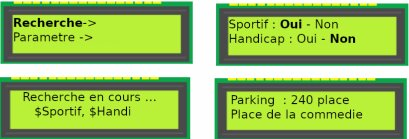
\includegraphics[width=0.9\textwidth]{UI.jpg}
\caption{Interface utilisateur}
\label{fig:universe}
\end{figure}

\section{Déterminer l'aspect matériel du dispositif}
 
 Pour un tel objet, nous pouvons facilement imaginer que nous allons l'utiliser dans notre voiture, et donc qu'un alume-cigare voir un port USB pourra faire office d'alimentation. 
 Comme nous allons utiliser un ESP32 pour notre microcontroleur, nous nous efforcerons de trouvé des modules GPS, ainsi que des modules 4G avec des bibliothèques existantes.
 Le GPS que nous utiliserons sera le REYAX RY8253F qui s'utilise facilement via un port serie. 
 Pour la puce 4G, des shields pour arduino existe donc supposera que nous pourrons utilser la connectivité de la meme maniere que pour la puce Wifi de l'ESP32.\\
 Pour la partie Interface utilisateur, nous utiliserons un ecran LCD 16x2 et 5 boutons pour faire notre ``joystick''
 Le montage resemblerait à celui ci :\\
 \begin{figure}[h!]
\centering
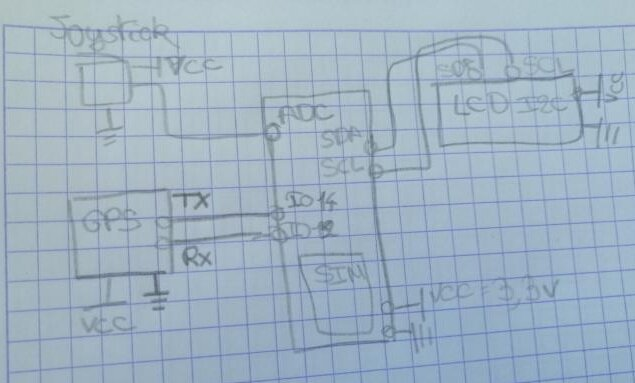
\includegraphics[width=0.9\textwidth]{2.jpg}
\caption{Montage}
\label{fig:universe}
\end{figure}\\
Pour ce qui est du joystick, on pourrait utilisé un montage comme celui ci, pour avoir : droite gauche, haut bas et le clique:\\
\begin{figure}[h!]
\centering
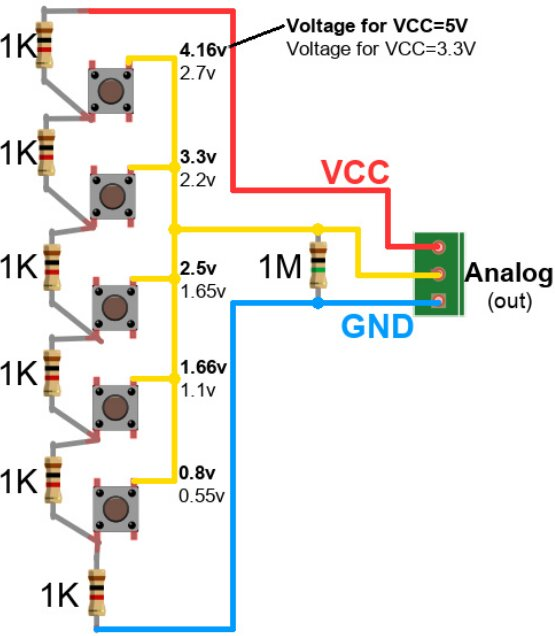
\includegraphics[width=0.5\textwidth]{3.jpg}
\caption{joystick}
\label{fig:universe}
\end{figure}
 \newpage

\section{Décrire de manière globale le fonctionnement logiciel}
 Voici comment le logiciel fonctionnera :
 
 \insertcode{code/pseudocode}{pseudocode}
 
 
 
 




\end{document}

